\chapter{Kết quả thực nghiệm và đánh giá}

Chương này tổng hợp các kết quả thực nghiệm được ghi nhận trong tài liệu kết quả của dự án, bao gồm kết quả của pipeline dữ liệu, mô hình Recall, mô hình Ranking và pipeline phục vụ suy luận. Các số liệu trong chương được dùng để phản ánh kết quả đã được ghi nhận trước đó, không phải số liệu suy diễn từ hình minh họa. Khi cần tái lập kết quả trên một môi trường mới, cần chạy lại đầy đủ pipeline dữ liệu, huấn luyện Recall, huấn luyện Ranking và kiểm thử API theo các lệnh ở Phụ lục.

\section{Kết quả pipeline dữ liệu}
Sau khi chạy pipeline dữ liệu, dữ liệu thô được chuyển đổi thành các tập dữ liệu phục vụ huấn luyện và phục vụ suy luận. Pipeline thực hiện lần lượt các bước đọc dữ liệu, biến đổi giá sản phẩm, chia phiên người dùng, tạo snapshot đặc trưng, tạo đặc trưng theo thời điểm (point-in-time features) và gán nhãn cho dữ liệu tương tác. Kết quả đầu ra chính gồm \texttt{labeled\_sessions.parquet}, \texttt{user\_features.parquet} và \texttt{item\_features.parquet}.
\medskip

Tập \texttt{labeled\_sessions.parquet} là dữ liệu huấn luyện đã được xử lý ở mức phiên-người dùng-sản phẩm. Điều này có nghĩa là nếu trong cùng một phiên, một người dùng tương tác nhiều lần với cùng một sản phẩm, hệ thống chỉ giữ lại dòng đại diện có tín hiệu mạnh nhất. Cách làm này giúp giảm trùng lặp và làm cho dữ liệu huấn luyện phản ánh rõ hơn mức độ quan tâm của người dùng đối với sản phẩm.
\medskip

Hai tập \texttt{user\_features.parquet} và \texttt{item\_features.parquet} được sử dụng như kho đặc trưng dạng snapshot. \texttt{user\_features.parquet} lưu các đặc trưng tổng hợp theo người dùng, chẳng hạn tổng số tương tác và tổng số phiên. \texttt{item\_features.parquet} lưu các đặc trưng tổng hợp theo sản phẩm, bao gồm số lượt tương tác, số người dùng duy nhất, giá trung bình, thông tin danh mục, thương hiệu và độ phổ biến theo phiên.

\section{Kết quả Recall}
Mô hình Recall được huấn luyện bằng Matrix Factorization với số chiều embedding là 64, kích thước batch là 4096, learning rate là 0.01 và số epoch là 5. Dữ liệu huấn luyện được cân bằng tương đối bằng lấy mẫu âm (negative sampling) với tỷ lệ 1 mẫu tích cực đi kèm tối đa 4 mẫu tiêu cực. Hàm mất mát được sử dụng là Focal Loss nhằm giảm ảnh hưởng của dữ liệu mất cân bằng.
\medskip

Theo kết quả thực nghiệm được ghi nhận trong tài liệu của dự án, giá trị mất mát (loss) của mô hình Recall giảm nhanh qua các epoch. Ở epoch đầu tiên, loss còn ở mức 0.0433. Sau 5 epoch, loss giảm xuống 0.0010. Điều này cho thấy mô hình học được mối quan hệ giữa người dùng và sản phẩm trên tập dữ liệu huấn luyện. Bảng~\ref{tab:recall_result} trình bày các giá trị cụ thể, còn Hình~\ref{fig:recall_loss_curve} giúp quan sát xu hướng giảm loss trực quan hơn.

\begin{table}[H]
\centering
\caption{Kết quả huấn luyện và đánh giá mô hình Recall}
\label{tab:recall_result}
\renewcommand{\arraystretch}{1.25}
\begin{tabularx}{\textwidth}{lcl}
\toprule
\textbf{Chỉ số} & \textbf{Giá trị} & \textbf{Nhận xét} \\
\midrule
Loss epoch 1 & 0.0433 & Mô hình bắt đầu học quan hệ người dùng-sản phẩm \\
Loss epoch 2 & 0.0320 & Loss tiếp tục giảm \\
Loss epoch 3 & 0.0097 & Mô hình hội tụ nhanh hơn \\
Loss epoch 4 & 0.0022 & Loss tiến gần mức thấp \\
Loss epoch 5 & 0.0010 & Loss tiếp tục giảm trên dữ liệu huấn luyện \\
Hit Rate@50 & 97.88\% & Ghi nhận 601/614 tương tác tích cực trong đánh giá \\
\bottomrule
\end{tabularx}
\end{table}

\begin{figure}[H]
\centering
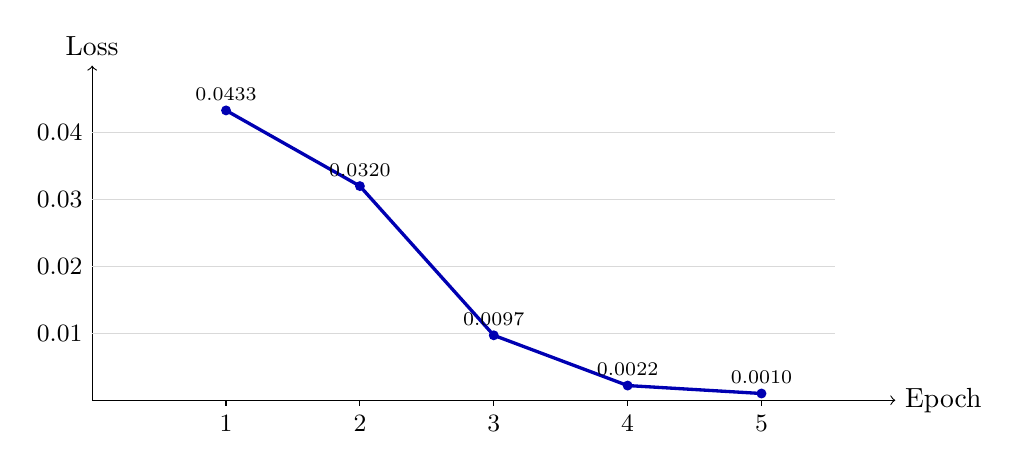
\begin{tikzpicture}[x=1.7cm,y=85cm]
    \draw[->] (0,0) -- (6.0,0) node[right] {Epoch};
    \draw[->] (0,0) -- (0,0.050) node[above] {Loss};
    \foreach \x/\label in {1/1,2/2,3/3,4/4,5/5} {
        \draw (\x,0) -- (\x,-0.0008) node[below] {\small \label};
    }
    \foreach \y/\label in {0.01/0.01,0.02/0.02,0.03/0.03,0.04/0.04} {
        \draw[gray!30] (0,\y) -- (5.55,\y);
        \node[left] at (0,\y) {\small \label};
    }
    \draw[blue!70!black, very thick] plot coordinates {
        (1,0.0433) (2,0.0320) (3,0.0097) (4,0.0022) (5,0.0010)
    };
    \foreach \x/\y/\v in {1/0.0433/0.0433,2/0.0320/0.0320,3/0.0097/0.0097,4/0.0022/0.0022,5/0.0010/0.0010} {
        \fill[blue!70!black] (\x,\y) circle (1.8pt);
        \node[above] at (\x,\y) {\scriptsize \v};
    }
\end{tikzpicture}
\caption{Đường giảm loss của mô hình Recall qua 5 epoch}
\label{fig:recall_loss_curve}
\end{figure}

Hình~\ref{fig:recall_loss_curve} cho thấy loss giảm mạnh nhất trong ba epoch đầu và tiếp tục giảm ở hai epoch cuối với biên độ nhỏ hơn. Kết quả Hit Rate@50 đạt 97.88\%, tương ứng 601 trên 614 tương tác tích cực được tìm thấy trong Top-50 ứng viên theo tài liệu ghi nhận của dự án. Chỉ số này cho thấy mô hình Recall có khả năng bao phủ tốt các sản phẩm liên quan trong điều kiện đánh giá đã ghi nhận. Tuy nhiên, cần lưu ý rằng kết quả Recall rất cao cũng có thể phản ánh nguy cơ đánh giá lạc quan vì hàm \texttt{evaluate\_recall()} trong \texttt{src/recall\_model/run\_recall.py} đang đánh giá trên các tương tác dương lấy từ cùng tập dữ liệu đã dùng để tạo vocabulary và huấn luyện, chưa phải một tập kiểm thử Recall tách biệt theo thời gian. Vì vậy, khi phát triển tiếp, nên đánh giá Recall trên tập kiểm thử tách theo thời gian để phản ánh chính xác hơn khả năng khái quát.

\section{Kết quả Ranking}
Mô hình Ranking được đánh giá bằng ba chỉ số chính: AUC, NDCG@10 và MRR. AUC phản ánh khả năng phân biệt giữa mẫu tích cực và mẫu không tích cực \cite{fawcett2006roc}. NDCG@10 đánh giá chất lượng thứ tự của 10 sản phẩm đầu tiên, trong đó các sản phẩm phù hợp xuất hiện ở vị trí cao sẽ có đóng góp lớn hơn \cite{jarvelin2002cumulated}. MRR đo vị trí của sản phẩm phù hợp đầu tiên trong danh sách, từ đó phản ánh mức độ nhanh chóng mà người dùng có thể nhìn thấy sản phẩm liên quan \cite{craswell2009mrr}.
\medskip

Dự án có hai hướng huấn luyện Ranking: mô hình cơ sở (baseline) và mô hình Train-on-Recall. Mô hình baseline được huấn luyện trực tiếp trên dữ liệu tương tác đã gán nhãn, sau khi ghép với đặc trưng người dùng và đặc trưng sản phẩm. Mô hình Train-on-Recall được huấn luyện trên tập ứng viên sinh ra từ chính pipeline Recall, nhờ đó dữ liệu huấn luyện gần hơn với dữ liệu mà Ranking gặp khi phục vụ suy luận. Bảng~\ref{tab:ranking_comparison} và Hình~\ref{fig:ranking_metrics_comparison} được dùng để so sánh hai hướng huấn luyện này.

\begin{table}[H]
\centering
\caption{Bảng so sánh hiệu năng xếp hạng giữa Baseline và Train-on-Recall}
\label{tab:ranking_comparison}
\renewcommand{\arraystretch}{1.25}
\small
\begin{tabularx}{\textwidth}{Xccc}
\toprule
\textbf{Mô hình} & \textbf{AUC} & \textbf{NDCG@10} & \textbf{MRR} \\
\midrule
Baseline & 0.6375 & 0.0495 & 0.0458 \\
Train-on-Recall & \textbf{0.9601} & \textbf{0.0653} & \textbf{0.0572} \\
\bottomrule
\end{tabularx}
\end{table}

\begin{figure}[H]
\centering
\begin{tikzpicture}[x=2.15cm,y=4.0cm]
    \draw[->] (0,0) -- (4.2,0) node[right] {Chỉ số};
    \draw[->] (0,0) -- (0,1.08) node[above] {Giá trị};
    \foreach \y in {0.2,0.4,0.6,0.8,1.0} {
        \draw[gray!30] (0,\y) -- (3.8,\y);
        \node[left] at (0,\y) {\small \y};
    }
    \foreach \x/\name/\b/\t in {
        0.9/AUC/0.6375/0.9601,
        2.0/NDCG@10/0.0495/0.0653,
        3.1/MRR/0.0458/0.0572
    } {
        \fill[gray!55] (\x-0.22,0) rectangle (\x-0.02,\b);
        \fill[blue!70!black] (\x+0.02,0) rectangle (\x+0.22,\t);
        \node[below] at (\x,0) {\small \name};
        \node[above] at (\x-0.12,\b) {\scriptsize \b};
        \node[above] at (\x+0.12,\t) {\scriptsize \t};
    }
    \fill[gray!55] (1.05,1.02) rectangle (1.25,1.07);
    \node[right] at (1.28,1.045) {\small Baseline};
    \fill[blue!70!black] (2.1,1.02) rectangle (2.3,1.07);
    \node[right] at (2.33,1.045) {\small Train-on-Recall};
\end{tikzpicture}
\caption{So sánh AUC, NDCG@10 và MRR giữa Baseline và Train-on-Recall}
\label{fig:ranking_metrics_comparison}
\end{figure}

Kết quả trong Hình~\ref{fig:ranking_metrics_comparison} cho thấy Train-on-Recall cải thiện đáng kể so với baseline. AUC tăng từ 0.6375 lên 0.9601, cho thấy mô hình phân biệt tốt hơn giữa ứng viên có tương tác và ứng viên không có tương tác. NDCG@10 tăng từ 0.0495 lên 0.0653, còn MRR tăng từ 0.0458 lên 0.0572. Mức tăng của NDCG và MRR cho thấy thứ tự hiển thị của danh sách gợi ý đã được cải thiện, dù giá trị tuyệt đối vẫn chưa cao.
\medskip

Việc NDCG@10 và MRR còn thấp là điều có thể giải thích được trong bối cảnh dữ liệu thương mại điện tử. Dữ liệu có độ thưa cao và tỷ lệ mẫu tích cực trong tập kiểm thử rất nhỏ. Khi nhiều nhóm người dùng hoặc phiên không có mẫu tích cực, các chỉ số xếp hạng trung bình sẽ bị kéo xuống. Do đó, các giá trị NDCG và MRR cần được đọc cùng với bối cảnh mất cân bằng dữ liệu, thay vì chỉ đánh giá theo độ lớn tuyệt đối.

\section{Kết quả phục vụ suy luận}
Kết quả phục vụ suy luận được đánh giá thông qua thời gian khởi tạo pipeline và độ trễ khi xử lý request gợi ý. Khi API khởi động, hệ thống cần nạp kho đặc trưng, encoder, item embedding, FAISS index, trọng số mô hình Recall và mô hình LightGBM. Đây là chi phí xảy ra một lần khi server khởi động, không phải chi phí của từng request.
\medskip

Đối với request gợi ý, hệ thống ghi nhận độ trễ của từng thành phần trong pipeline. Các thành phần chính gồm lấy user embedding, truy vấn FAISS, tra cứu kho đặc trưng, chấm điểm LightGBM, sắp xếp kết quả và tạo response. Tài liệu thực nghiệm của dự án ghi nhận độ trễ tổng hợp khoảng 22.5 ms trong môi trường cục bộ. Bảng~\ref{tab:serving_latency} và Hình~\ref{fig:serving_latency_breakdown} trình bày cách phân rã độ trễ theo từng thành phần.

\begin{table}[H]
\centering
\caption{Bảng tổng hợp độ trễ tham chiếu của pipeline phục vụ}
\label{tab:serving_latency}
\renewcommand{\arraystretch}{1.25}
\small
\begin{tabularx}{\textwidth}{Xcc}
\toprule
\textbf{Thành phần} & \textbf{Thời gian} & \textbf{Tỷ trọng} \\
\midrule
Tra cứu đặc trưng & 2.8 ms & 12.4\% \\
Tìm kiếm FAISS & 4.5 ms & 20.0\% \\
Xếp hạng LightGBM & 12.2 ms & 54.2\% \\
Sắp xếp và tạo phản hồi & 3.0 ms & 13.4\% \\
\midrule
\textbf{Tổng độ trễ} & \textbf{22.5 ms} & \textbf{100\%} \\
\bottomrule
\end{tabularx}
\end{table}

\begin{figure}[H]
\centering
\begin{tikzpicture}[x=1.65cm,y=0.22cm]
    \draw[->] (0,0) -- (5.6,0) node[right] {Thành phần};
    \draw[->] (0,0) -- (0,14.2) node[above] {ms};
    \foreach \y in {0,3,6,9,12} {
        \draw[gray!30] (0,\y) -- (5.2,\y);
        \node[left] at (0,\y) {\small \y};
    }
    \fill[green!55!black] (0.52,0) rectangle (1.08,2.8);
    \node[align=center, below] at (0.8,0) {\scriptsize Tra cứu\\\scriptsize đặc trưng};
    \node[above] at (0.8,2.8) {\scriptsize 2.8 ms};
    \fill[blue!65] (1.72,0) rectangle (2.28,4.5);
    \node[align=center, below] at (2.0,0) {\scriptsize FAISS};
    \node[above] at (2.0,4.5) {\scriptsize 4.5 ms};
    \fill[purple!65] (2.92,0) rectangle (3.48,12.2);
    \node[align=center, below] at (3.2,0) {\scriptsize LightGBM};
    \node[above] at (3.2,12.2) {\scriptsize 12.2 ms};
    \fill[orange!75] (4.12,0) rectangle (4.68,3.0);
    \node[align=center, below] at (4.4,0) {\scriptsize Sắp xếp\\\scriptsize phản hồi};
    \node[above] at (4.4,3.0) {\scriptsize 3.0 ms};
\end{tikzpicture}
\caption{Biểu đồ phân rã độ trễ theo bảng tổng hợp pipeline phục vụ}
\label{fig:serving_latency_breakdown}
\end{figure}

Hình~\ref{fig:serving_latency_breakdown} cho thấy giai đoạn xếp hạng bằng LightGBM có thể chiếm tỷ trọng đáng kể trong tổng thời gian xử lý vì mô hình phải chấm điểm nhiều ứng viên cùng lúc. Tuy nhiên, các benchmark cho từng yêu cầu cụ thể trong tài liệu dự án cũng ghi nhận rằng tỷ trọng từng thành phần có thể thay đổi theo kịch bản. Với truy vấn chỉ dùng kênh dài hạn, tổng độ trễ được ghi nhận khoảng 35.23 ms; với truy vấn hai kênh có \texttt{session\_items}, tổng độ trễ được ghi nhận khoảng 16.97 ms. Trong các lần đo này, thời gian tra cứu đặc trưng có thể lớn hơn thời gian chấm điểm LightGBM. Vì vậy, có thể kết luận rằng API đạt mục tiêu dưới 50 ms trong các kịch bản thử nghiệm cục bộ đã ghi nhận, còn nút thắt hiệu năng cụ thể phụ thuộc vào dữ liệu, trạng thái bộ nhớ và loại yêu cầu.

\section{Nhận xét và hạn chế}
Từ các kết quả thực nghiệm, có thể thấy hệ thống đã xây dựng được một pipeline gợi ý tương đối hoàn chỉnh. Mô hình Recall giúp thu hẹp nhanh không gian tìm kiếm sản phẩm, trong khi FAISS bảo đảm quá trình truy hồi ứng viên diễn ra với độ trễ thấp. Mô hình Ranking giúp cải thiện chất lượng danh sách cuối cùng bằng cách sắp xếp lại các ứng viên theo nhiều nhóm đặc trưng khác nhau.
\medskip

Dù vậy, hệ thống vẫn còn một số hạn chế. Kho đặc trưng hiện tại là các file Parquet được nạp vào RAM, phù hợp với môi trường thực nghiệm nhưng chưa phải là giải pháp tối ưu cho hệ thống lớn hoặc dữ liệu thay đổi liên tục. Hệ thống cũng chưa có cơ chế cập nhật dữ liệu theo thời gian thực. Ngoài ra, đánh giá Recall cần được tách huấn luyện/kiểm thử chặt chẽ hơn để tránh kết quả quá lạc quan, còn mô hình Ranking hiện vẫn dùng binary objective thay vì tối ưu trực tiếp cho mục tiêu xếp hạng.
